\documentclass[a4paper,12pt]{report}
\usepackage[left=1.1in, right=1.1in, top=1in, bottom=1.18in]{geometry}
\usepackage{amsmath}
\usepackage{enumerate}
\usepackage{enumitem}
\usepackage{latexsym}
\usepackage{caption}
\usepackage{subcaption}
%\useunder{\uline}{\ul}{}
\usepackage[table,xcdraw]{xcolor}
\tolerance=1
\emergencystretch=\maxdimen
\hyphenpenalty=10000
\hbadness=10000

\usepackage{fancyhdr}

\usepackage{setspace}
%\usepackage{epsfig}

\usepackage{tocloft}

\usepackage[pdftex]{graphicx}
\thispagestyle{empty}
\onehalfspacing

%%Front Page
\begin{document}
	\begin{center}
		\vspace{12pt}
		\Large\textbf{M.Sc.}
		\Large\textbf{(Five Year Integrated) in}
		\Large\textbf{Computer Science  (Artificial Intelligence \& Data Science)\\}
		\vspace{30pt}
		\Large\textbf{Third Semester}
		\vspace*{50pt}
		\textbf{\\ Laboratory Record}
		\vspace{5pt}
		
		\Large\textbf{21-805-0307: DATABASE SYSTEMS LAB\\ }
		\vspace*{40pt}
		\small\textit{\textbf{Submitted in partial fulfillment\\ of the requirements for the award of degree in \\ Master of Science (Five Year Integrated)\\in Computer Science (Artificial Intelligence \& Data Science) of \\ Cochin University of Science and Technology (CUSAT) \\ Kochi\\ }}
		\vspace*{10pt}
		\begin{center}
		
\includegraphics[scale=0.5]{cusat.png}	
		\end{center}
		
		\vspace*{0pt}
		\begin{center}
		\textbf{\textit{Submitted by\hspace{350pt}}}
		\end{center}

%%Type your name and Reg No here

		\textbf{AKSHAY K S\hspace{600pt}}
		\vspace*{20pt}
		\textbf{(80521005) \hspace{300pt}}
		\vspace*{0pt}
		\small\textbf{DEPARTMENT OF COMPUTER SCIENCE\\}
		\small\textbf{COCHIN UNIVERSITY OF SCIENCE AND TECHNOLOGY (CUSAT)\\}
		\small\textbf{KOCHI-682022\\}
		\vspace{10pt}
		\small\textbf{JANUARY 2023}
		
		
		
	\end{center}
	\newpage
	\thispagestyle{empty}
	
	%%CERTIFICATE PAGE
	
	\begin{center}
		\large\textbf{DEPARTMENT OF COMPUTER SCIENCE\\}
		\small\textbf{COCHIN UNIVERSITY OF SCIENCE AND TECHNOLOGY (CUSAT)\\}
		\small\textbf{KOCHI, KERALA-682022\\}
		\vspace*{20pt}
		
\includegraphics[scale=0.5]{cusat.png}
		\vspace*{20pt}
	\end{center}
	\vspace{15pt}
	%%Edit your name and Register Number
	
	\textit{This is to certify that the software laboratory record for \textbf{21-805-0307: Database Systems Lab} is a record of work carried out by \textbf{AKSHAY K S(80521005)}, in partial fulfillment of the requirements for the award of degree in \textbf{Master of Science\small\text{ (Five Year Integrated)}} \normalsize in \textbf{Computer Science (Artificial Intelligence \& Data Science)} of Cochin University of Science and Technology (CUSAT), Kochi. The lab record has been approved as it satisfies the academic requirements in respect of the second semester laboratory prescribed for the Master of Science (Five Year Integrated) in Computer Science degree.\\\\\\\\\\\ }
	\vspace{50pt}
	\small\textbf{Faculty Member in-charge\\}
	\vspace{0pt}
	Sajmi Salaam \hspace{275pt} Dr. Philip Samuel \\
	Guest Faculty \hspace{267 pt} Professor and Head\\
	Department of Computer Science \hspace{106pt} Department of Computer Science \\
	CUSAT \hspace{352pt} CUSAT
	

	\newpage
	
	\pagenumbering{roman}
    \setcounter{page}{1}


	
	\pagestyle{fancy}
	\fancyhead[L]{\footnotesize{21-805-0307: Database Systems Lab}}
	\fancyfoot[C]{}
	\fancyfoot[L]{\footnotesize{Dept. of Computer Science, CUSAT}}
	\fancyfoot[R]{\footnotesize{Page \thepage}}
		
\begin{table}[!h]
\renewcommand{\arraystretch}{1.69}
\resizebox{\columnwidth}{!}{
%\small\addtolength{\tabcolsep}{-1pt}
\begin{tabular}{lll} &
  \multicolumn{1}{c}{\textbf{Table of Contents}} &
   \\ \hline
 
\rowcolor[HTML]{FFFFFF} 
{\color[HTML]{000000} \textbf{Sl.No.}} &
  \multicolumn{1}{c}{\cellcolor[HTML]{FFFFFF}{\color[HTML]{000000} \textbf{Program}}} &
  {\color[HTML]{000000} \textbf{Page.No.}} \\

  \hline
\rowcolor[HTML]{FFFFFF} 
\multicolumn{1}{|l|}{\cellcolor[HTML]{FFFFFF}{\color[HTML]{000000} 1}} &
  \multicolumn{1}{l|}{\cellcolor[HTML]{FFFFFF}{\color[HTML]{000000}Schema Diagram and ER Diagram}} &
  \multicolumn{1}{l|}{\cellcolor[HTML]{FFFFFF}{\color[HTML]{000000} 1}} \\ \hline
\rowcolor[HTML]{FFFFFF} 
\multicolumn{1}{|l|}{\cellcolor[HTML]{FFFFFF}{\color[HTML]{000000} 2}} &
  \multicolumn{1}{l|}{\cellcolor[HTML]{FFFFFF}{\color[HTML]{000000} Queries to implement DDL Commands}} &
  \multicolumn{1}{l|}{\cellcolor[HTML]{FFFFFF}{\color[HTML]{000000} 2}} \\ \hline
\rowcolor[HTML]{FFFFFF} 
\multicolumn{1}{|l|}{\cellcolor[HTML]{FFFFFF}{\color[HTML]{000000} 3}} &
  \multicolumn{1}{l|}{\cellcolor[HTML]{FFFFFF}{\color[HTML]{000000} Queries to implement DML Commands}}&
  \multicolumn{1}{l|}{\cellcolor[HTML]{FFFFFF}{\color[HTML]{000000} 6}} \\ \hline
\multicolumn{1}{|l|}{4} &
  \multicolumn{1}{l|}{Queries to implement DCL Commands.} &
  \multicolumn{1}{l|}{11} \\ \hline
\multicolumn{1}{|l|}{5} &
  \multicolumn{1}{l|}{{Queries to implement Group Functions}} &
  \multicolumn{1}{l|}{12} \\ \hline
\multicolumn{1}{|l|}{6} &
  \multicolumn{1}{l|}{Program to implement Nested Queries} &
  \multicolumn{1}{l|}{15} \\ \hline
\multicolumn{1}{|l|}{7} &
  \multicolumn{1}{l|}{Program to implement Views} &
  \multicolumn{1}{l|}{26} \\ \hline
\multicolumn{1}{|l|}{8} &
  \multicolumn{1}{l|}{Programs of Functions And Procedures} &
  \multicolumn{1}{l|}{29} \\ \hline
\multicolumn{1}{|l|}{9} &
  \multicolumn{1}{l|}{Implementation of Cursor} &
  \multicolumn{1}{l|}{32} \\ \hline
\multicolumn{1}{|l|}{10} &
  \multicolumn{1}{l|}{Implementation of Trigger} &
  \multicolumn{1}{l|}{35} \\ \hline
\multicolumn{1}{|l|}{11} &
  \multicolumn{1}{l|}{\cellcolor[HTML]{FFFFFF}{\color[HTML]{24292F} Queries to implement TCL Commands}} &
  \multicolumn{1}{l|}{41} \\ \hline
\multicolumn{1}{|l|}{12} &
  \multicolumn{1}{l|}{\cellcolor[HTML]{FFFFFF}{\color[HTML]{24292F} Operations on NOSQL Systems}} &
  \multicolumn{1}{l|}{\cellcolor[HTML]{FFFFFF}{\color[HTML]{24292F} 44}} \\ \hline
\multicolumn{1}{|l|}{13} &
  \multicolumn{1}{l|}{Simple Structure of GraphQL program} &
  \multicolumn{1}{l|}{47} \\ \hline
\multicolumn{1}{|l|}{14} &
  \multicolumn{1}{l|}{Programs demonstrating Java Database Connectivity} &
  \multicolumn{1}{l|}{52} \\ \hline
\multicolumn{1}{|l|}{15} &
  \multicolumn{1}{l|}{Project Report on Application Software} &
  \multicolumn{1}{l|}{52} \\ \hline
  
\end{tabular}}
\end{table}


	%%To include the chapter name in the index page add the following comment after /newpage with program title

	\newpage
	\pagenumbering{arabic}
	\setcounter{page}{1}	
\newpage
	%%To include the chapter name in the index page add the following comment after /newpage with program title
	
%%%%%%%%%%%%%%%%%%%%%%%%%%%%%%%%%%%%%%%%%%%%%%%%%%%%%%%%%%%%

\begin{center}
		%%Title of the Program
		\large\textbf{SCHEMA DIAGRAM}
	\end{center}
\paragraph{}
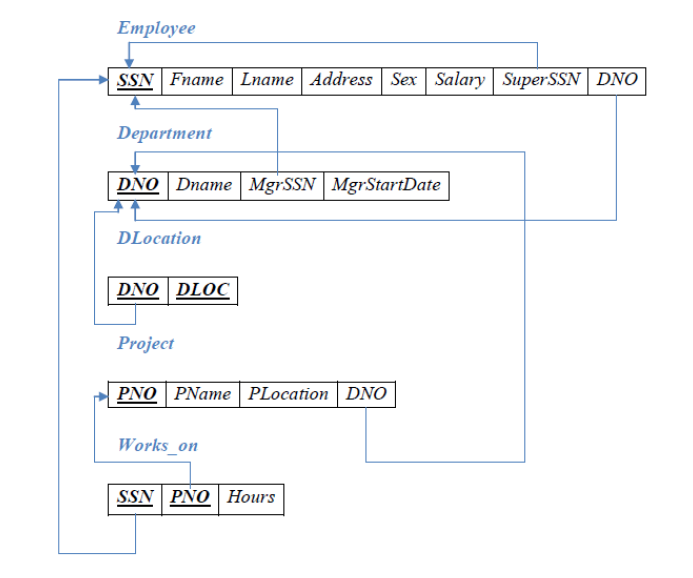
\includegraphics[scale=0.5]{SCHEMA.png}


\begin{center}
		%%Title of the Program
		\large\textbf{ER DIAGRAM}
	\end{center}
\paragraph{}
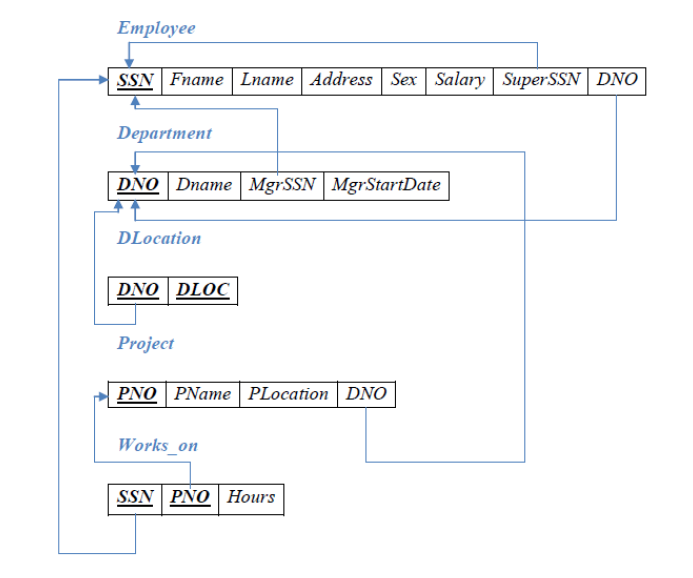
\includegraphics[scale=0.5]{SCHEMA.png}
 \newpage

%%%%%%%%%%%%%%%%%%%%%%%%%%
	\begin{center}
		%%Title of the Program
		\large\textbf{DDL COMMANDS}
	\end{center}
	
	\begin{flushleft}
		\textbf{AIM }
	\end{flushleft} 
%%Insert AIM of your program here
	    Develop SQL Queries to execute and verify the Data Definition Language commands and also implement Data Constraints.
\begin{flushleft}
    \textbf{Questions : 1}
\end{flushleft}
 Create five tables using constraints like primary key, not null, check, default, null, unique, foreign key  as per the above schema
	
	\begin{flushleft}
		\textbf{QUERY }
	\end{flushleft}
%%Insert the program code here
\begin{verbatim}
mysql> use COMPANY;
Database changed

mysql> create table EMPLOYEE(SSN varchar(50) primary key not null,Fname 
varchar(30),Lname varchar(30) null,Address varchar(50),Sex varchar(20)
default 'Male',Salary int(30) check(Salary>10000),SuperSSN varchar(20)
unique,DNO varchar(20));

Query OK, 0 rows affected, 1 warning (0.02 sec)

mysql> create table DEPARTMENT(DNO varchar(20) primary key,Dname varchar(20),
MgrSSN varchar(20), MgrStartData date not null);

Query OK, 0 rows affected (0.01 sec)

mysql> create table PROJECT(PNO varchar(20) primary key,PName varchar(30),
PLocation varchar(20),DNO varchar(20),constraint dno_project foreign key(DNO) 
references DEPARTMENT(DNO));

Query OK, 0 rows affected (0.02 sec)

mysql> create table WORKS_ON(SSN varchar(20) primary key,PNO varchar(20),
Hours integer);

Query OK, 0 rows affected (0.01 sec)

mysql> create table DLOCATION(DNO varchar(20) primary key,DLOC varchar(20));

Query OK, 0 rows affected (0.01 sec)

mysql> desc EMPLOYEE;

Query OK, 0 rows affected (0.01 sec)

mysql> desc DEPARTMENT;

Query OK, 0 rows affected (0.01 sec)

mysql> desc PROJECT;

Query OK, 0 rows affected (0.01 sec)

mysql> desc WORKS_ON;

Query OK, 0 rows affected (0.01 sec)

mysql> desc DLOCATION;

Query OK, 0 rows affected (0.01 sec)

\end{verbatim}

	\begin{flushleft}
		\textbf{DATABASE TABLES}
	\end{flushleft} 
%%Insert screen shot of sample output as image file as filename.png
      \includegraphics[scale=0.6]{employee.png}
    \includegraphics[scale=0.6]{department.png}
    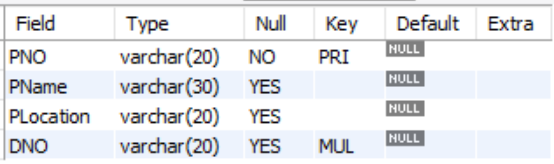
\includegraphics[scale=1.3]{PROJECT.png}
    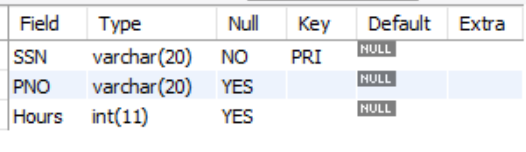
\includegraphics[scale=1.3]{WORKS_ON.png}
	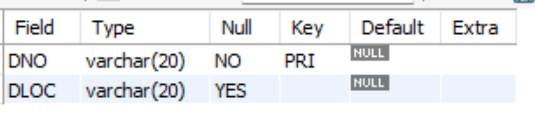
\includegraphics[scale=1.3]{DLOCATION.png}
	\newpage
	
%%%%%%%%%%%%%%%%%%%%%%%%%%%%%%%%%%%%%%%%%%%%%%%%%%

\begin{flushleft}
    \textbf{Questions : 2}
\end{flushleft}
Add another column Age with datatype integer in employee table
\begin{flushleft}
		\textbf{QUERY }
	\end{flushleft}
%%Insert the program code here
\begin{verbatim}
mysql> alter table EMPLOYEE add(AGE integer);

Query OK, 0 rows affected (0.02 sec)
Records: 0  Duplicates: 0  Warnings: 0

\end{verbatim}

\begin{flushleft}
		\textbf{DATABASE TABLES}
\end{flushleft} 

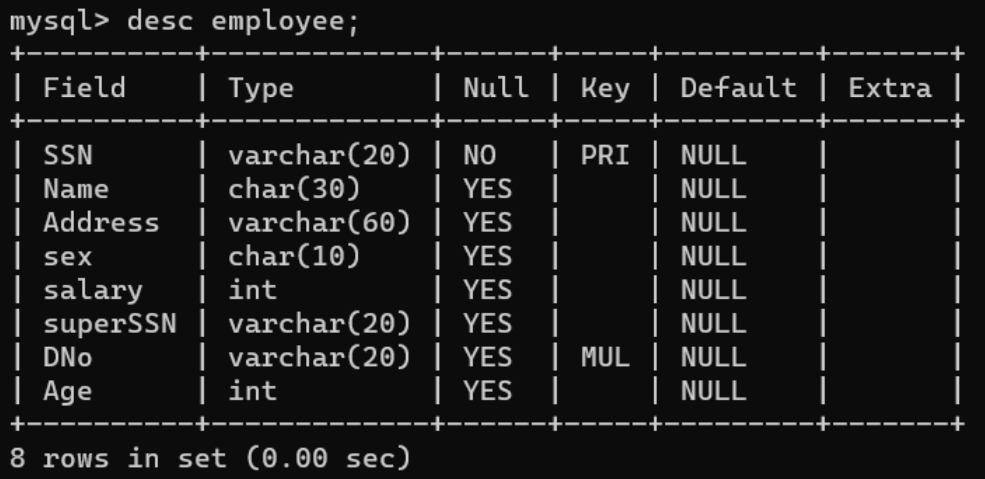
\includegraphics[scale=0.7]{ALTER_ADD.png}
\begin{flushleft}
    \textbf{Questions : 3}
\end{flushleft}
Drop a table named Project
\begin{flushleft}
		\textbf{QUERY }
	\end{flushleft}
%%Insert the program code here
\begin{verbatim}
mysql> DROP TABLE PROJECT;

Query OK, 0 rows affected (0.01 sec)

\end{verbatim}

\begin{flushleft}
		\textbf{DATABASE TABLES}
\end{flushleft} 

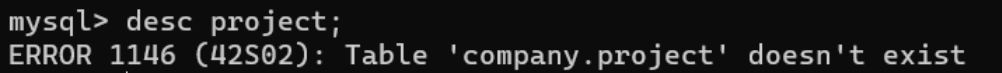
\includegraphics[scale=0.8]{DROP.png}
	\newpage
%%%%%%%%%%%%%%%%%%%%%%%%%%%%%%%%%%%%%%%%%%%%%%%%%%%%%%%%%%%%
\begin{flushleft}
    \textbf{Questions : 4}
\end{flushleft}
Truncate a table named WORKS\_ON
\begin{flushleft}
		\textbf{QUERY }
	\end{flushleft}
%%Insert the program code here
\begin{verbatim}
mysql> TRUNCATE TABLE WORKS_ON;

Query OK, 0 rows affected (0.01 sec)

\end{verbatim}

\begin{flushleft}
		\textbf{DATABASE TABLES}
\end{flushleft} 

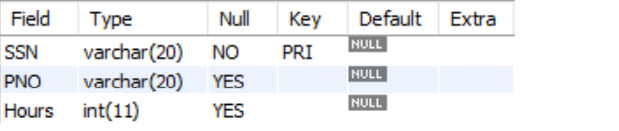
\includegraphics[scale=1.1]{TRUNCATE.png}
\begin{flushleft}
    \textbf{Questions : 5}
\end{flushleft}
View the structure of the table Department
\begin{flushleft}
		\textbf{QUERY }
	\end{flushleft}
%%Insert the program code here
\begin{verbatim}
mysql> DESC DEPARTMENT;

\end{verbatim}

\begin{flushleft}
		\textbf{DATABASE TABLES}
\end{flushleft} 

\includegraphics[scale=0.6]{department.png}

\newpage
%%%%%%%%%%%%%%%%%%%%%%%%%%%%%%%%%%%%%%%%%%%%%%%%%%%%%%%%%%%
\begin{center}
		%%Title of the Program
		\large\textbf{DML COMMANDS}
	\end{center}
	
	\begin{flushleft}
		\textbf{AIM }
	\end{flushleft} 
%%Insert AIM of your program here
	   Develop SQL Queries to execute and verify the Data Manipulation Language commands.
\begin{flushleft}
    \textbf{Questions : 1}
\end{flushleft}
 Insert five records in the tables as per the above schema
	
	\begin{flushleft}
		\textbf{QUERY }
	\end{flushleft}
%%Insert the program code here
\begin{verbatim}
mysql> insert into EMPLOYEE values ("e1001","Raj","Sharma","Mumbai","Male",
15000,"s1001","d01",22);
Query OK, 1 row affected (0.00 sec)

mysql> insert into EMPLOYEE values ("e1002","Ria","Chopra","Chennai","Female",
20000,"s1002","d02",22);
Query OK, 1 row affected (0.01 sec)

mysql> insert into EMPLOYEE values ("e1003","Hira","Mohammed","Kochi","Female",
17000,"s1003","d03",20);
Query OK, 1 row affected (0.00 sec)

mysql> insert into EMPLOYEE values ("e1004","Simran","S","Chennai","Female",
15000,"s1004","d04",21); 
Query OK, 1 row affected (0.01 sec)

mysql> insert into EMPLOYEE values ("e1005","Ashwin","K","Mumbai","Male",
25000,"s1005","d05",21);
Query OK, 1 row affected (0.00 sec)

mysql> insert into DEPARTMENT values("d01","Marketing","m1001","2022-07-04");;
Query OK, 1 row affected (0.00 sec)

mysql> insert into DEPARTMENT values("d02","Finance","m1002","2022-04-07");
Query OK, 1 row affected (0.00 sec)

mysql> insert into DEPARTMENT values("d03","Sales","m1003","2022-08-18");
Query OK, 1 row affected (0.00 sec)

mysql> insert into DEPARTMENT values("d04","Human Resources","m1004","2022-02-1
7");
Query OK, 1 row affected (0.01 sec)

mysql> insert into DEPARTMENT values("d05","Management","m1005","2021-12-17");
Query OK, 1 row affected (0.00 sec)

mysql> insert into PROJECT values("p1001","Project Synergy","Chennai","d01");
Query OK, 1 row affected (0.01 sec)

mysql> insert into PROJECT values ("p1002","Project Point","Mumbai","d02");
Query OK, 1 row affected (0.00 sec)

mysql> insert into PROJECT values ("p1003","Strategic Program","Delhi","d03");
Query OK, 1 row affected (0.00 sec)

mysql> insert into PROJECT values ("p1004","Apollo","Mumbai","d04");
Query OK, 1 row affected (0.01 sec)

mysql> insert into PROJECT values ("p1005","Astron","Chennai","d05");
Query OK, 1 row affected (0.01 sec)

mysql> insert into WORKS_ON values("e1001","p1001",7);
Query OK, 1 row affected (0.00 sec)

mysql> insert into WORKS_ON values("e1002","p1002",10);
Query OK, 1 row affected (0.00 sec)

mysql> insert into WORKS_ON values("e1003","p1003",9);
Query OK, 1 row affected (0.00 sec)

mysql> insert into WORKS_ON values("e1004","p1004",10);
Query OK, 1 row affected (0.00 sec)

mysql> insert into WORKS_ON values("e1005","p1005",4);
Query OK, 1 row affected (0.01 sec)

mysql> insert into DLOCATION values("d01","Chennai");
Query OK, 1 row affected (0.00 sec)

mysql> insert into DLOCATION values("d02","Mumbai");
Query OK, 1 row affected (0.00 sec)

mysql> insert into DLOCATION values("d03","Delhi");
Query OK, 1 row affected (0.01 sec)

mysql> insert into DLOCATION values("d04","Mumbai");
Query OK, 1 row affected (0.01 sec)

mysql> insert into DLOCATION values("d05","Chennai");
Query OK, 1 row affected (0.01 sec)
\end{verbatim}

\begin{flushleft}
    \textbf{Questions : 2}
\end{flushleft}
Display the entire content of the tables as per the above schema
\begin{flushleft}
		\textbf{QUERY }
	\end{flushleft}
%%Insert the program code here
\begin{verbatim}
mysql> SELECT * FROM EMPLOYEE;
mysql> SELECT * FROM DEPARTMENT;
mysql> SELECT * FROM PROJECT;
mysql> SELECT * FROM WORKS_ON;
mysql> SELECT * FROM DLOCATION;

\end{verbatim}

\begin{flushleft}
		\textbf{DATABASE TABLES}
\end{flushleft} 

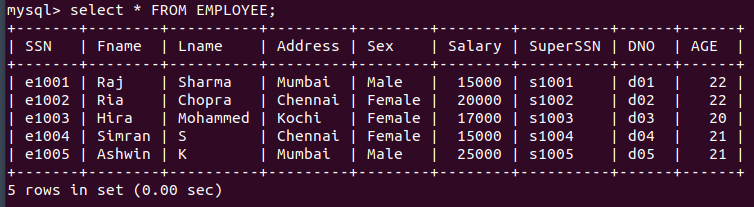
\includegraphics[scale=0.5]{EMPLOYEE2.png}\newline\newline
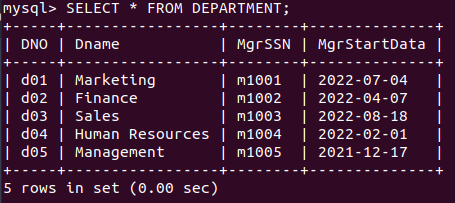
\includegraphics[scale=0.8]{DEPARTMENT2.png}\newline\newline
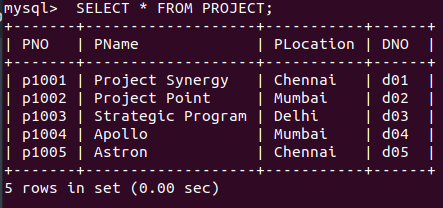
\includegraphics[scale=0.7]{PROJECT2.png}\newline\newline
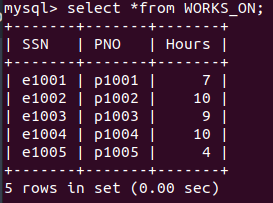
\includegraphics[scale=0.8]{WORKS_ON2.png}\newline\newline
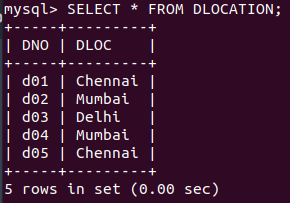
\includegraphics[scale=0.8]{DLOCATION2.png}\\

\begin{flushleft}
    \textbf{Questions : 3}
\end{flushleft}
Modify the salary of the employee as 25000 whose SSN is e1001
\begin{flushleft}
		\textbf{QUERY }
	\end{flushleft}
%%Insert the program code here
\begin{verbatim}
mysql> Update EMPLOYEE set SALARY=25000 where SSN="e1002";
Query OK, 1 row affected (0.00 sec)
Rows matched: 1  Changed: 1  Warnings: 0

\end{verbatim}


\begin{flushleft}
		\textbf{DATABASE TABLES} 
\end{flushleft} 

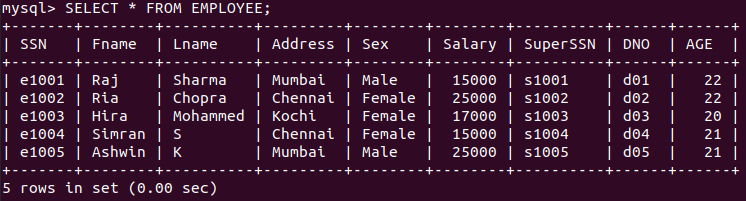
\includegraphics[scale=0.5]{UPDATE.png}

\begin{flushleft}
    \textbf{Questions : 4}
\end{flushleft}
Delete the details of the employee whose SSN is "e1002"
\begin{flushleft}
		\textbf{QUERY }
	\end{flushleft}
%%Insert the program code here
\begin{verbatim}
mysql> Update EMPLOYEE set SALARY=25000 where SSN="e1002";
Query OK, 1 row affected (0.00 sec)
Rows matched: 1  Changed: 1  Warnings: 0

\end{verbatim}


\begin{flushleft}
		\textbf{DATABASE TABLES} 
\end{flushleft} 

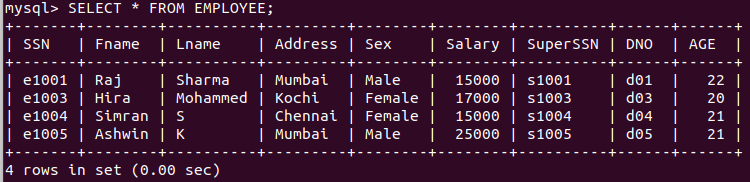
\includegraphics[scale=0.5]{DELETE.png}
\newpage
%%%%%%%%%%%%%%%%%%%%%%%%%%%%%%%%%%%%%%%%%%%%%%%%%%%%%%%%
\begin{center}
		%%Title of the Program
		\large\textbf{DCL COMMANDS}
	\end{center}
	
	\begin{flushleft}
		\textbf{AIM }
	\end{flushleft} 
%%Insert AIM of your program here
	   Develop SQL Queries to implement Data Control Language commands
\begin{flushleft}
    \textbf{Questions : 1}
\end{flushleft}
 To grant a SELECT permission on employee table to user1
	
	\begin{flushleft}
		\textbf{QUERY }
	\end{flushleft}
%%Insert the program code here
\begin{verbatim}
mysql> create user 'user1'@'localhost' identified by 'password';
Query OK, 0 rows affected (0.01 sec)

mysql> grant select on COMPANY.EMPLOYEE to 'user1'@'localhost';
Query OK, 0 rows affected (0.01 sec)

\end{verbatim}
\begin{flushleft}
		\textbf{DATABASE TABLES} 
\end{flushleft} 

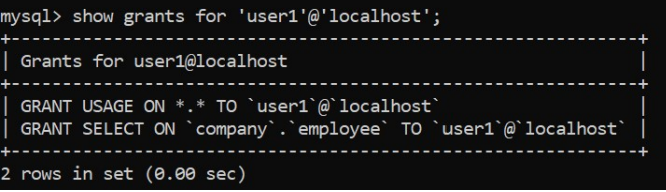
\includegraphics[scale=1.1]{SELECT.png}

\begin{flushleft}
    \textbf{Questions : 2}
\end{flushleft}
Revoking a privilege to all users in a table
	\begin{flushleft}
		\textbf{QUERY }
	\end{flushleft}
%%Insert the program code here
\begin{verbatim}
mysql> grant all on COMPANY.EMPLOYEE to 'user1'@'localhost';
Query OK, 0 rows affected (0.01 sec)

mysql> Revoke all on EMPLOYEE from 'user1'@'localhost';
Query OK, 0 rows affected (0.00 sec)

\end{verbatim}
\begin{flushleft}
		\textbf{DATABASE TABLES} 
\end{flushleft} 

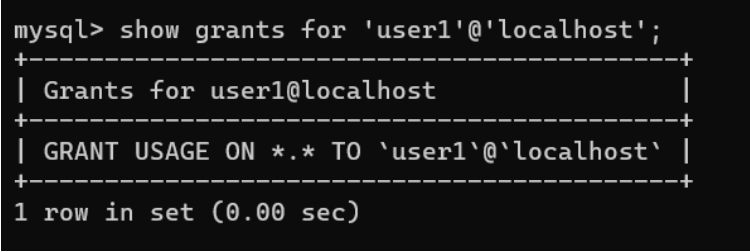
\includegraphics[scale=1.1]{REVOKE.png}
\newpage
%%%%%%%%%%%%%%%%%%%%%%%%%%%%%%%%%%%%%%%%%%%%%%%%%%%%%%%%%%%%
\begin{center}
		%%Title of the Program
		\large\textbf{GROUP FUNCTION OR AGGREGATE FUNCTION}
	\end{center}
	
	\begin{flushleft}
		\textbf{AIM }
	\end{flushleft} 
%%Insert AIM of your program here
	   Develop SQL Queries to execute computation on table data with built-in functions
\begin{flushleft}
    \textbf{Questions : 1}
\end{flushleft}
List the fname of all the employee having ‘a’ as the second last character in their name.	
	\begin{flushleft}
		\textbf{QUERY }
	\end{flushleft}
 \begin{verbatim}
     mysql> select Fname from EMPLOYEE where Fname like '%a_';
 \end{verbatim}
\begin{flushleft}
		\textbf{DATABASE TABLES} 
\end{flushleft} 

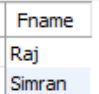
\includegraphics[scale=1.2]{Q1.png}
\begin{flushleft}
    \textbf{Questions : 2}
\end{flushleft}
Count the total number of male and female employees in the Employee table.
	\begin{flushleft}
		\textbf{QUERY }
	\end{flushleft}
 \begin{verbatim}
   mysql> select Sex,count(*) from EMPLOYEE group by Sex;  
 \end{verbatim}
\begin{flushleft}
		\textbf{DATABASE TABLES} 
\end{flushleft} 

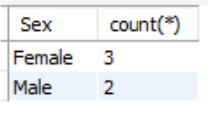
\includegraphics[scale=1.2]{Q2.png}
\begin{flushleft}
    \textbf{Questions : 3}
\end{flushleft}
Calculate the average salary of  the  female employees.
	\begin{flushleft}
		\textbf{QUERY }
	\end{flushleft}
 \begin{verbatim}
 mysql> select avg(Salary) from EMPLOYEE where Sex="Female";    
 \end{verbatim}
\begin{flushleft}
		\textbf{DATABASE TABLES} 
\end{flushleft} 

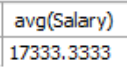
\includegraphics[scale=1.2]{Q3.png}
\begin{flushleft}
    \textbf{Questions : 4}
\end{flushleft}
Calculate the sum of salaries of male employees.
	\begin{flushleft}
		\textbf{QUERY }
	\end{flushleft}
 \begin{verbatim}
     mysql> select sum(Salary) from EMPLOYEE where Sex="Male";
 \end{verbatim}
\begin{flushleft}
		\textbf{DATABASE TABLES} 
\end{flushleft} 

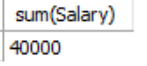
\includegraphics[scale=1.2]{Q4.png}
\begin{flushleft}
    \textbf{Questions : 5}
\end{flushleft}
Display the maximum and minimum salaries of male employees.
	\begin{flushleft}
		\textbf{QUERY }
	\end{flushleft}
 \begin{verbatim}
     mysql> select max(Salary),min(Salary) from EMPLOYEE where Sex="Male";
 \end{verbatim}
\begin{flushleft}
		\textbf{DATABASE TABLES} 
\end{flushleft} 

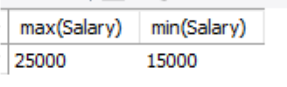
\includegraphics[scale=1.2]{Q5.png}

\begin{flushleft}
    \textbf{Questions : 6}
\end{flushleft}
Display the details of all employees whose salary between 25000 and 50000
	\begin{flushleft}
		\textbf{QUERY }
	\end{flushleft}
 \begin{verbatim}
     mysql> select * from EMPLOYEE where Salary between 25000 and 50000;
 \end{verbatim}
\begin{flushleft}
		\textbf{DATABASE TABLES} 
\end{flushleft} 

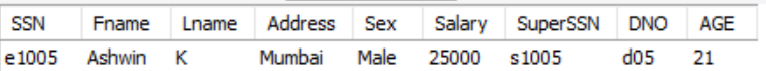
\includegraphics[scale=1.2]{Q6.png}

\begin{flushleft}
    \textbf{Questions : 7}
\end{flushleft}
Display the lname of the employees whose salaries are 30000 or 40000 or 50000.
	\begin{flushleft}
		\textbf{QUERY }
	\end{flushleft}
 \begin{verbatim}
    mysql> select Lname from EMPLOYEE where Salary=30000 or Salary=40000
    or Salary = 50000; 
 \end{verbatim}
\begin{flushleft}
		\textbf{DATABASE TABLES} 
\end{flushleft} 

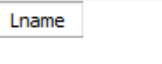
\includegraphics[scale=1.5]{Q7.png}

%%%%%%%%%%%%%%%%%%%%%%%%%%%%%%%%%%%%%%
\newpage
\begin{center}
		%%Title of the Program
		\large\textbf{NESTED QUERIES}
	\end{center}
	
	\begin{flushleft}
		\textbf{AIM }
	\end{flushleft} 
%%Insert AIM of your program here
	   Develop SQL Queries to implement Nested Queries/ Sub Queries and Joins

\begin{flushleft}
    \textbf{Questions : 1}
\end{flushleft}
Update the salary by 0.25 times for all the employees whose Plocation is ‘Chennai’.
	\begin{flushleft}
		\textbf{QUERY }
	\end{flushleft}
 \begin{verbatim}
 
mysql> Update EMPLOYEE,PROJECT set Salary=Salary+(Salary*0.25)/100 where 
EMPLOYEE.DNo=PROJECT.DNo and PLocation="Chennai";
Query OK, 2 rows affected (0.01 sec)
Rows matched: 2  Changed: 2  Warnings: 0
\end{verbatim}
\begin{flushleft}
		\textbf{DATABASE TABLES} 
\end{flushleft} 

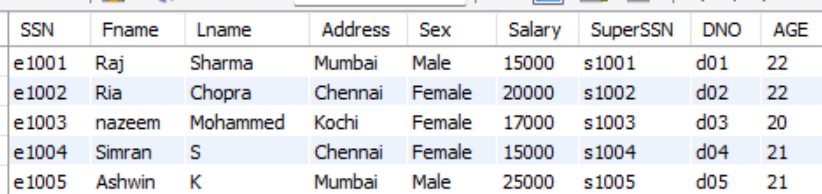
\includegraphics[scale=0.5]{NQ1.png}
\begin{flushleft}
    \textbf{Questions : 2}
\end{flushleft}

To display the name and project location of employees whose working hour is greater than 5
	\begin{flushleft}
		\textbf{QUERY }
	\end{flushleft}
 \begin{verbatim}
mysql> select EMPLOYEE.Fname,PROJECT.PLocation FROM EMPLOYEE,WORKS_ON,PROJECT 
where WORKS_ON.Hours > 5 and EMPLOYEE.SSN = WORKS_ON.SSN 
and WORKS_ON.PNo=PROJECT.PNo;
 \end{verbatim}
\begin{flushleft}
		\textbf{DATABASE TABLES} 
\end{flushleft} 
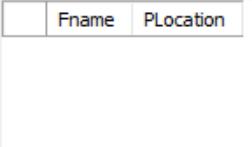
\includegraphics[scale=1]{NQ2.png}
\begin{flushleft}
    \textbf{Questions : 3}
\end{flushleft}
Left join employee table and works\_on table
	\begin{flushleft}
		\textbf{QUERY }
	\end{flushleft}
 \begin{verbatim}
mysql> select * from EMPLOYEE left join WORKS_ON on EMPLOYEE.SSN = WORKS_ON.SSN;
 \end{verbatim}
\begin{flushleft}
		\textbf{DATABASE TABLES} 
\end{flushleft} 

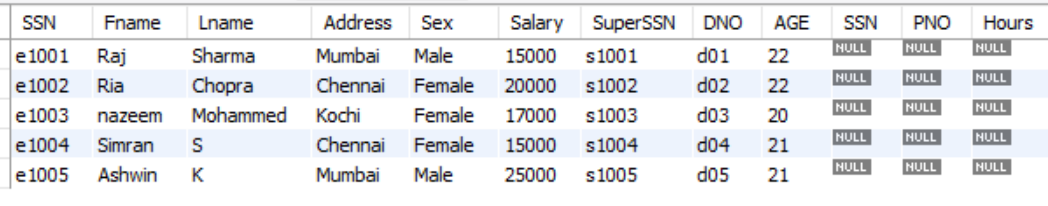
\includegraphics[scale=1]{NQ3.png}
\begin{flushleft}
    \textbf{Questions : 4}
\end{flushleft}
Right join works\_on table and employee table
	\begin{flushleft}
		\textbf{QUERY }
	\end{flushleft}
 \begin{verbatim}
 
mysql> select * from WORKS_ON RIGHT join EMPLOYEE on 
EMPLOYEE.SSN = WORKS_ON.SSN;

 \end{verbatim}
 
\begin{flushleft}
		\textbf{DATABASE TABLES} 
\end{flushleft} 

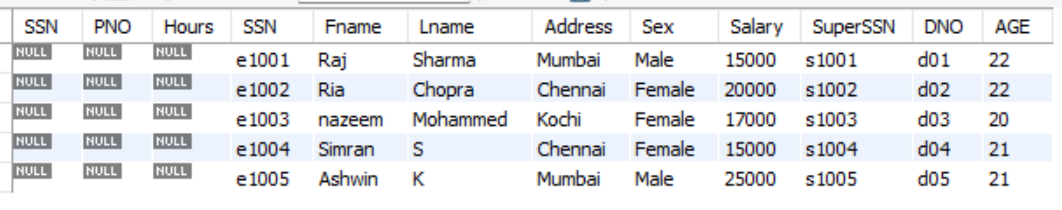
\includegraphics[scale=1]{NQ4.png}

\begin{flushleft}
    \textbf{Questions : 5}
\end{flushleft}

Full join works\_on table and employee table

	\begin{flushleft}
		\textbf{QUERY }
	\end{flushleft}
 \begin{verbatim}
 
mysql> select * from WORKS_ON full join EMPLOYEE ;

 \end{verbatim}
\begin{flushleft}
		\textbf{DATABASE TABLES} 
\end{flushleft} 

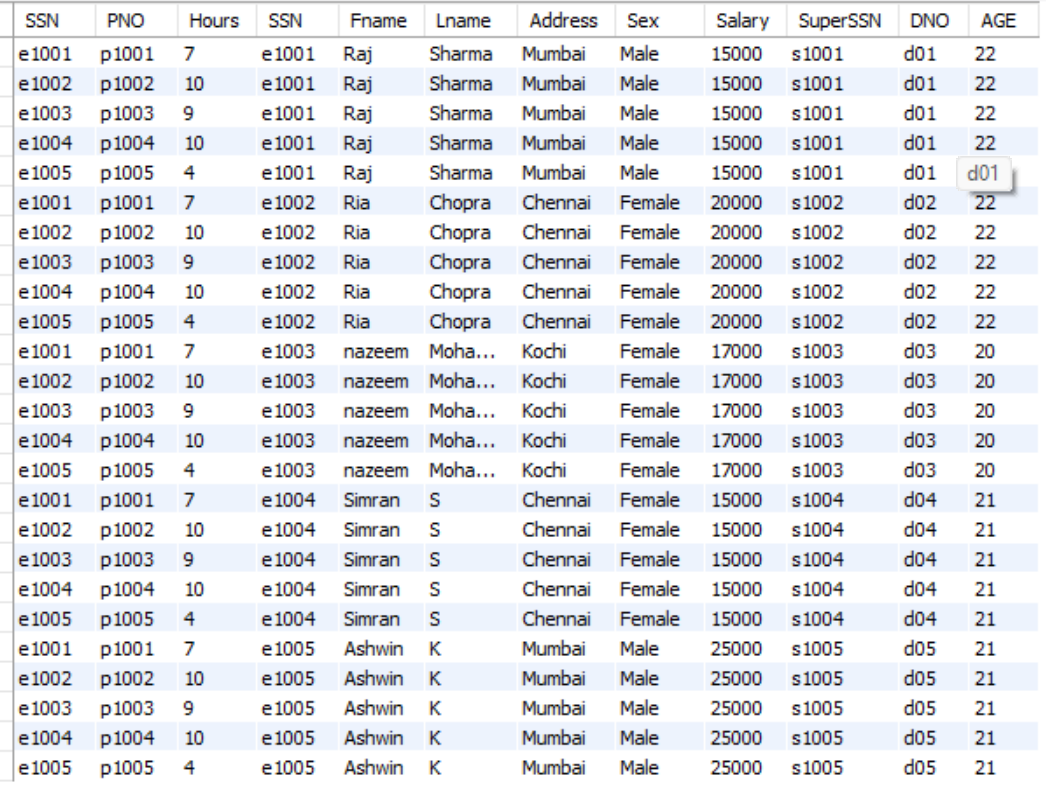
\includegraphics[scale=0.9]{NQ5.png}
%%%%%%%%%%%%%%%%%%%%%%%%%%%%%%%%%%%%%%
\newpage
\begin{center}
		%%Title of the Program
		\large\textbf{VIEWS}
	\end{center}
	
	\begin{flushleft}
		\textbf{AIM }
	\end{flushleft} 
%%Insert AIM of your program here
	   Develop SQL Queries for creating and dropping Views

\begin{flushleft}
    \textbf{Questions : 1}
\end{flushleft}
Create a view VW\_emp on employee table
	\begin{flushleft}
		\textbf{QUERY }
	\end{flushleft}
 \begin{verbatim}
 
mysql> create view VW_emp as select*from EMPLOYEE;
Query OK, 0 rows affected (0.00 sec)

\end{verbatim}
\begin{flushleft}
		\textbf{DATABASE TABLES} 
\end{flushleft} 

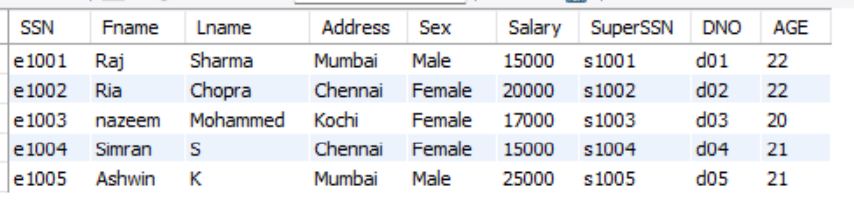
\includegraphics[scale=0.9]{VIEW1.png}
\begin{flushleft}
    \textbf{Questions : 2}
\end{flushleft}
Create another view VW\_SSN contains SuperSSN and Dno of female employees
	\begin{flushleft}
		\textbf{QUERY }
	\end{flushleft}
 \begin{verbatim}
 
mysql> create  view VW_SSN as select SuperSSN, DNO from EMPLOYEE 
where Sex = 'Female';
Query OK, 0 rows affected (0.01 sec)

\end{verbatim}
\begin{flushleft}
		\textbf{DATABASE TABLES} 
\end{flushleft} 

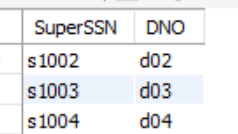
\includegraphics[scale=1]{VIEW2.png}
\begin{flushleft}
    \textbf{Questions : 3}
\end{flushleft}
Update the address of employee to Chennai whose id is e100 in view VW\_emp
	\begin{flushleft}
		\textbf{QUERY }
	\end{flushleft}
 \begin{verbatim}
 
mysql> UPDATE VW_emp SET Address="Chennai" WHERE SSN='e1001';
Query OK, 1 row affected (0.01 sec)
Rows matched: 1  Changed: 1  Warnings: 0


\end{verbatim}
\begin{flushleft}
		\textbf{DATABASE TABLES} 
\end{flushleft} 

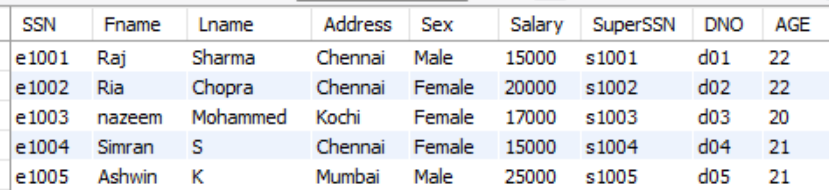
\includegraphics[scale=1]{VIEW3.png}
\begin{flushleft}
    \textbf{Questions : 4}
\end{flushleft}
Delete the view VW\_emp
	\begin{flushleft}
		\textbf{QUERY }
	\end{flushleft}
 \begin{verbatim}
 
mysql> drop view VW_emp;
Query OK, 0 rows affected (0.00 sec)

\end{verbatim}
\begin{flushleft}
		\textbf{DATABASE TABLES} 
\end{flushleft} 


\includegraphics[scale=0.8]{VIEW4.png}
%%%%%%%%%%%%%%%%%%%%%%%%%%%%%%%%%%%%%%
\newpage
\begin{center}
		%%Title of the Program
		\large\textbf{FUNCTIONS AND PROCEDURES}
	\end{center}
	
	\begin{flushleft}
		\textbf{AIM }
	\end{flushleft} 
%%Insert AIM of your program here
	   Develop PL/SQL program to familiarize with Function and Procedure

\begin{flushleft}
    \textbf{Questions : 1}
\end{flushleft}
Write a PL/SQL function to find factorial of a number
	\begin{flushleft}
		\textbf{QUERY }
	\end{flushleft}
 \begin{verbatim}
 
SQL*Plus: Release 11.2.0.2.0 Production on Fri Dec 16 14:29:44 2022

Copyright (c) 1982, 2014, Oracle.  All rights reserved.

SQL> connect
Enter user-name: system
Enter password:
Connected.


SQL> set serveroutput on
SQL> edit@factorial.sql

		create or replace function get_factorial(N int)
		return varchar
		is
		fact int := 1;
		begin
		for i in 1..N loop
		fact := fact*i;
		end loop;
		return 'Factorial is  '  || fact ;
		end;
		/
		select get_factorial(5) from dual;


SQL> @XEfactorial.sql

Function created.

\end{verbatim}
\begin{flushleft}
		\textbf{DATABASE TABLES} 
\end{flushleft} 

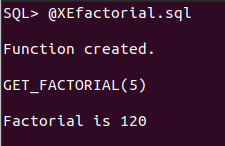
\includegraphics[scale=0.7]{FACTORIAL.png}


\begin{flushleft}
    \textbf{Questions : 2}
\end{flushleft}
Write a PL/SQL function to find maximum of two numbers
	\begin{flushleft}
		\textbf{QUERY }
	\end{flushleft}
 \begin{verbatim}
 
SQL*Plus: Release 11.2.0.2.0 Production on Fri Dec 16 14:29:44 2022

Copyright (c) 1982, 2014, Oracle.  All rights reserved.

SQL> connect
Enter user-name: system
Enter password:
Connected.


SQL> set serveroutput on
SQL> edit@max.sql

		create or replace function maximum(n1 int, n2 int)
		return varchar
		is
		m int := 0;
		begin
		if n1>n2 then 
		m := n1;
		else
		m := n2;
		end if;
		return  'Maximum is  ' ||m;
		end;
		/
		select maximum(4,9) from dual;

SQL> @XEmax.sql

Function created.

\end{verbatim}
\begin{flushleft}
		\textbf{DATABASE TABLES} 
\end{flushleft} 

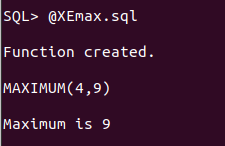
\includegraphics[scale=0.7]{MAXIMUM.png}


\begin{flushleft}
    \textbf{Questions : 3}
\end{flushleft}
Write a PL/SQL procedure to print the prime 
	\begin{flushleft}
		\textbf{QUERY }
	\end{flushleft}
 \begin{verbatim}
 
SQL*Plus: Release 11.2.0.2.0 Production on Fri Dec 16 14:29:44 2022

Copyright (c) 1982, 2014, Oracle.  All rights reserved.

SQL> connect
Enter user-name: system
Enter password:
Connected.


SQL> set serveroutput on

SQL> edit@prime.sql

		DECLARE
    			i NUMBER(3);
    			j NUMBER(3);
		BEGIN
		dbms_output.Put_line('The prime numbers are:');
				dbms_output.new_line;
    			i := 2;
    			LOOP
        			j := 2;
        			LOOP
            				EXIT WHEN( ( MOD(i, j) = 0 )
                        			OR ( j = i ) );
            				j := j + 1;
        			END LOOP;
        			IF( j = i )THEN
         				dbms_output.Put(i||'   ');		   
        			END IF;
        			i := i + 1;
        			exit WHEN i = 50;
    			END LOOP;
				dbms_output.new_line;
		END;
		/
		
SQL> @XEprime.sql

Function created.

\end{verbatim}
\begin{flushleft}
		\textbf{DATABASE TABLES} 
\end{flushleft} 

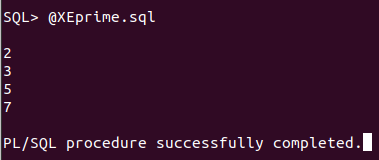
\includegraphics[scale=0.7]{PRIME.png}


\begin{flushleft}
    \textbf{Questions : 4}
\end{flushleft}
Write a PL/SQL procedure to display numbers from 1 to 10 using while loop
\begin{flushleft}
		\textbf{QUERY }
	\end{flushleft}
 \begin{verbatim}
 
SQL*Plus: Release 11.2.0.2.0 Production on Fri Dec 16 14:29:44 2022

Copyright (c) 1982, 2014, Oracle.  All rights reserved.

SQL> connect
Enter user-name: system
Enter password:
Connected.


SQL> set serveroutput on
SQL> edit@numbers.sql

		DECLARE
    			i INTEGER := 1;
		BEGIN
    			WHILE i <= 10 LOOP 
        			DBMS_OUTPUT.PUT_LINE(i);
    			i := i+1;
    			END LOOP;
		END;
		/

SQL> @XEnumbers.sql

Function created.

\end{verbatim}
\begin{flushleft}
		\textbf{DATABASE TABLES} 
\end{flushleft} 

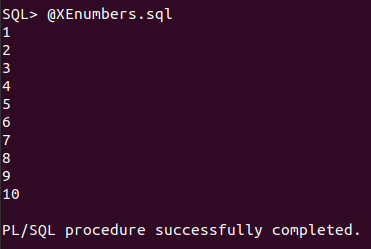
\includegraphics[scale=0.7]{NUMBERS.png}

%%%%%%%%%%%%%%%%%%%%%%%%%%%%%%%%%%%%%%
\newpage
\begin{center}
		%%Title of the Program
		\large\textbf{CURSOR}
	\end{center}
	
	\begin{flushleft}
		\textbf{AIM }
	\end{flushleft} 
%%Insert AIM of your program here
	 Develop PL/SQL program to implement Cursor

\begin{flushleft}
    \textbf{Questions : 1}
\end{flushleft}
Write a PL/SQL cursor program to update the salary of each employee of department number D001 in the Employee table as per the schema
	\begin{flushleft}
		\textbf{QUERY }
	\end{flushleft}
 \begin{verbatim}
SQL> declare cursor employee_cur is
  2  select SSN,Salary from Employee where DNO = 'D001'
  3  for update;
  4  incr_sal number;
  5  begin
  6  for employee_rec in employee_cur loop
  7  if employee_rec.Salary < 50000 then
  8  incr_sal := .15;
  9  else
 10  incr_sal := .10;
 11  end if;
 12  update Employee set Salary = Salary + Salary * incr_sal where current of
 employee_cur;
 13  end loop;
 14  end;
 15  /

PL/SQL procedure successfully completed.
\end{verbatim}
\begin{flushleft}
		\textbf{DATABASE TABLES} 
\end{flushleft} 

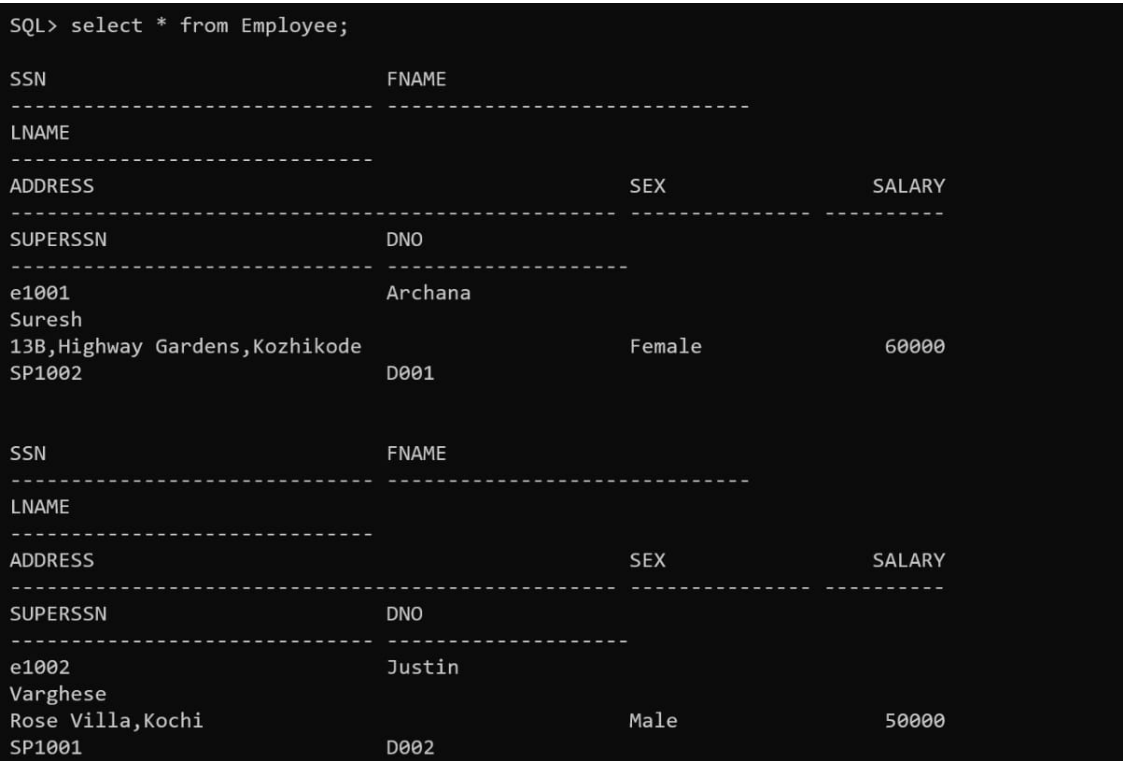
\includegraphics[scale=0.8]{CURSOR1.png}
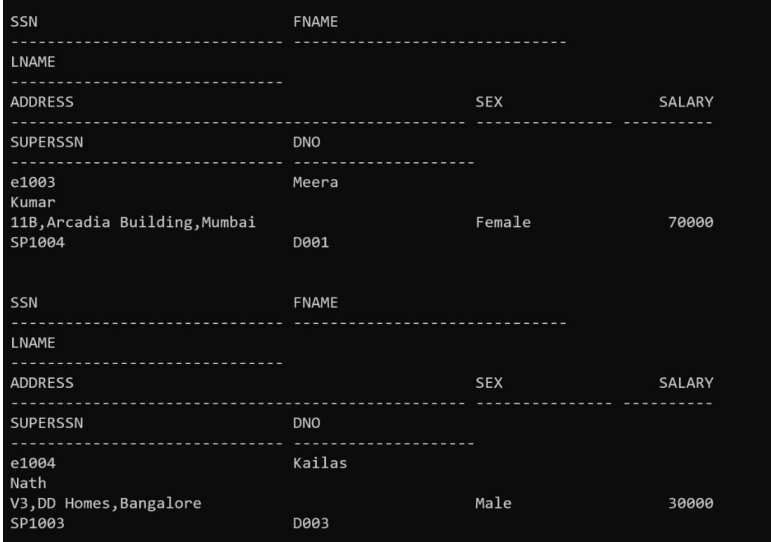
\includegraphics[scale=0.8]{CURSOR2.1.png}
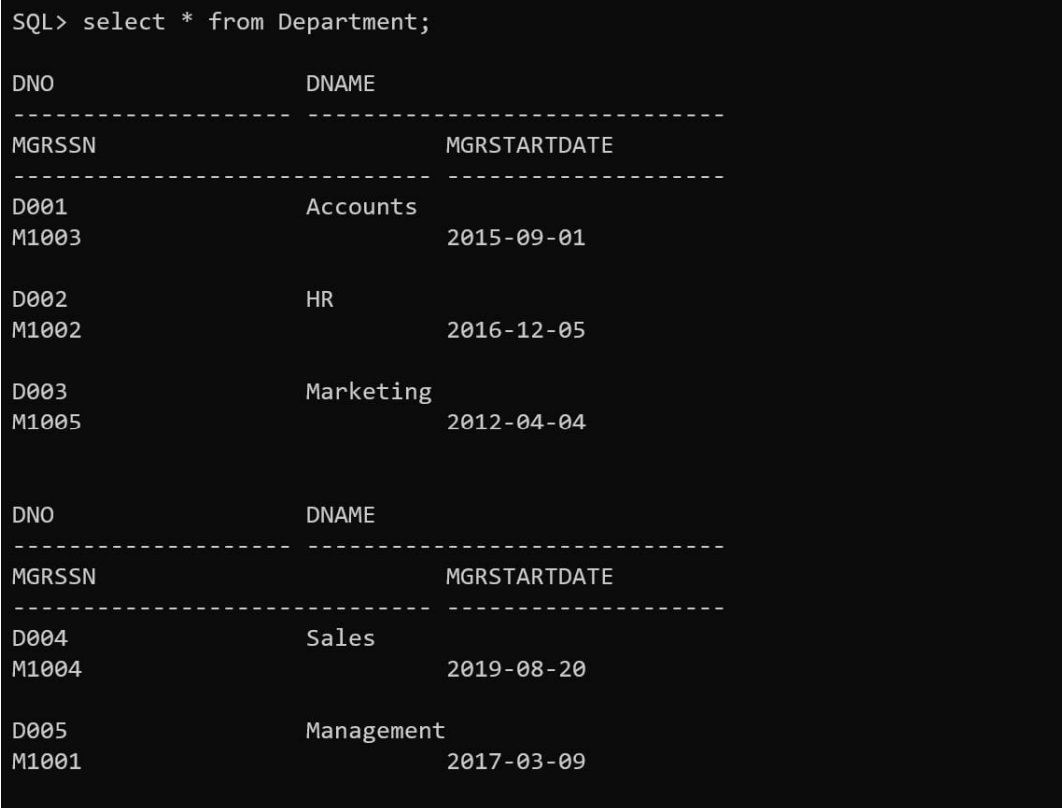
\includegraphics[scale=0.8]{CURSOR2.2.png}
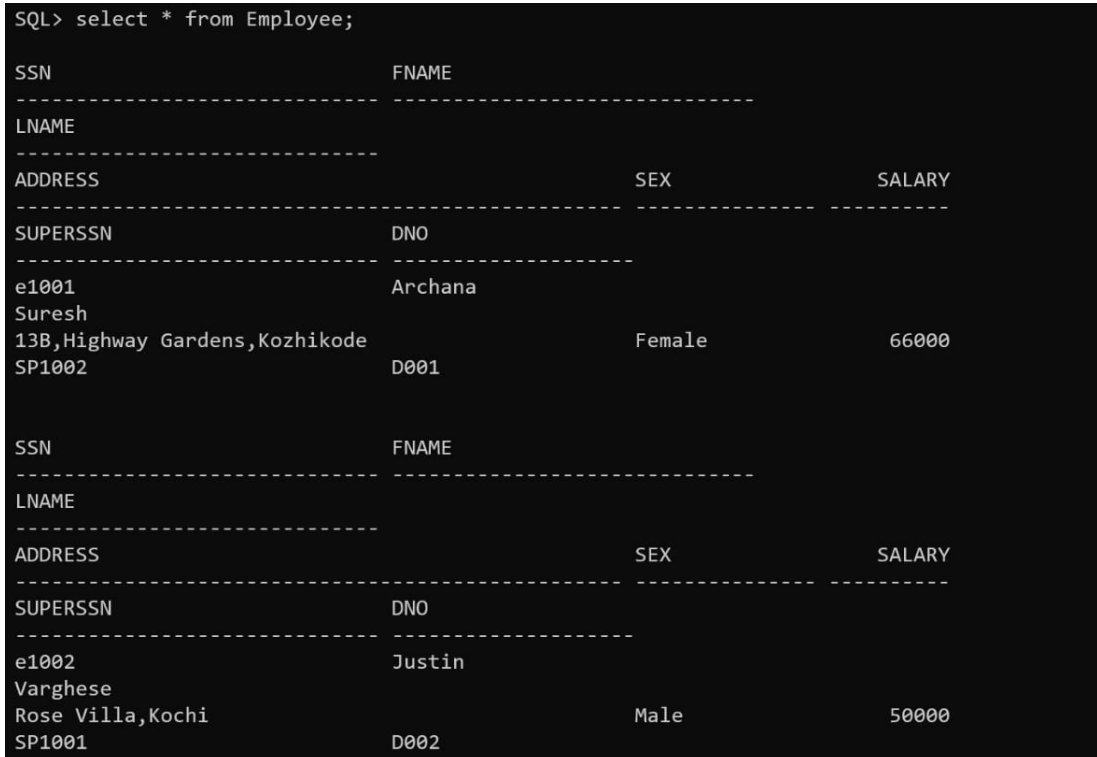
\includegraphics[scale=0.8]{CURSOR2.3.png}
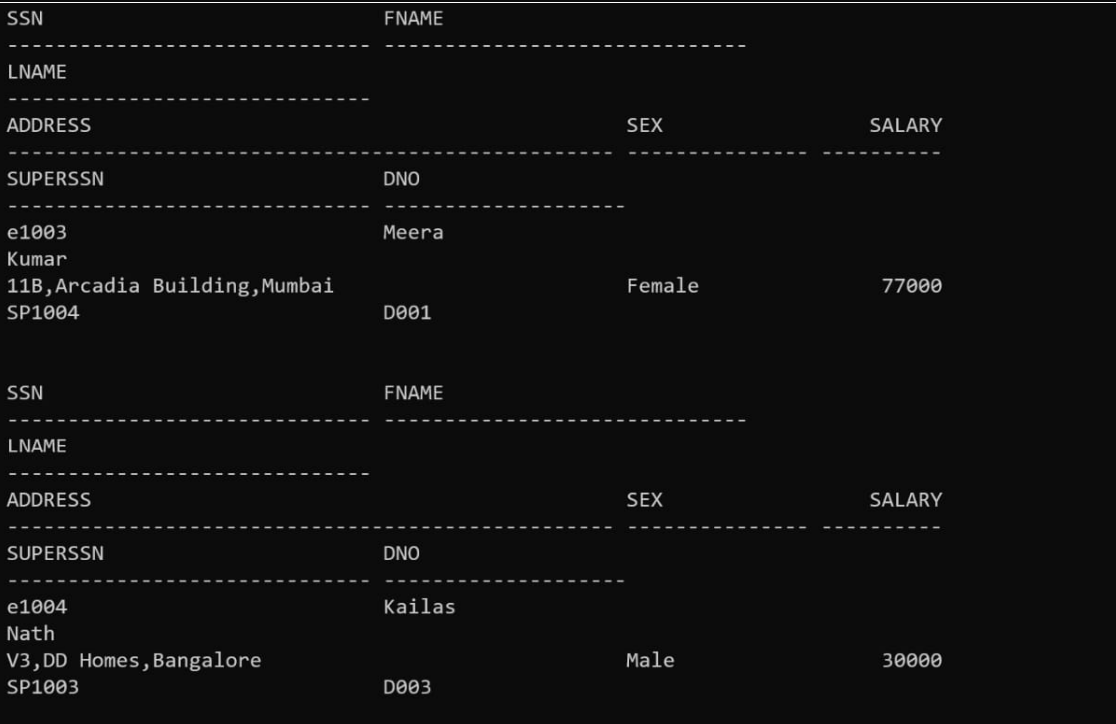
\includegraphics[scale=0.8]{CURSOR2.4.png}
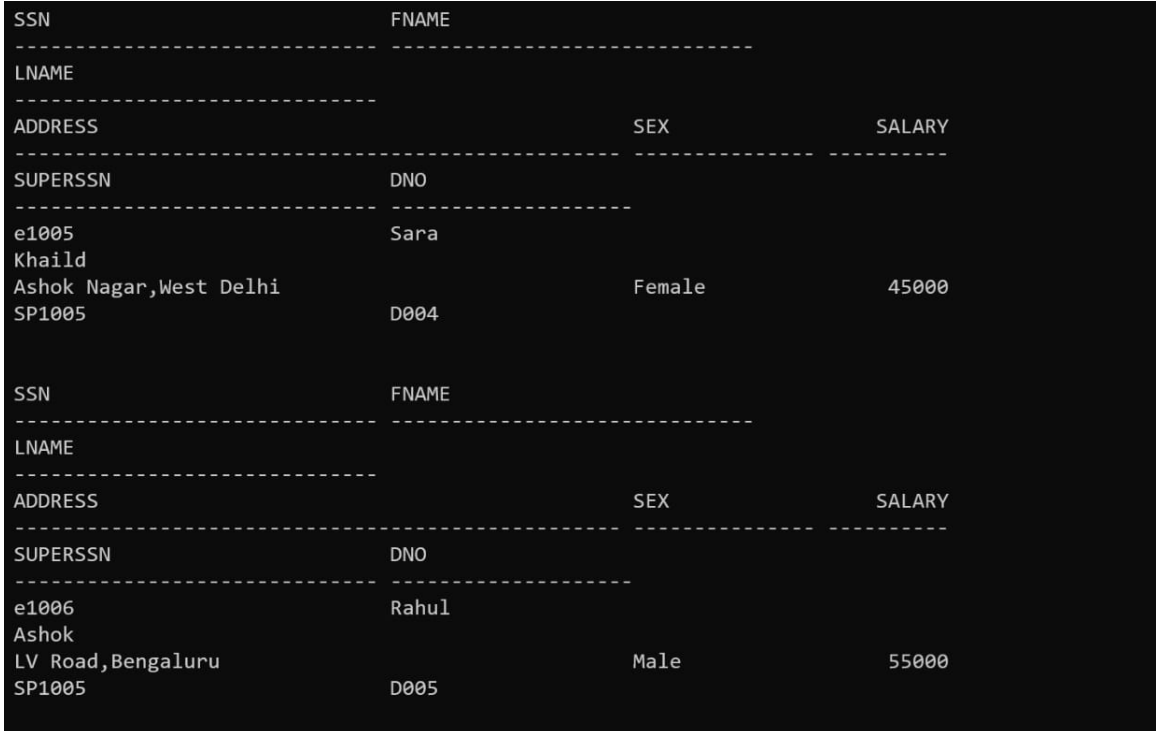
\includegraphics[scale=0.8]{CURSOR2.5.png}


\begin{flushleft}
    \textbf{Questions : 2}
\end{flushleft}
Write a PL/SQL cursor program to retrieve Dno and DName from Department table as per the schema
	\begin{flushleft}
		\textbf{QUERY }
	\end{flushleft}
 \begin{verbatim}
 SQL> declare cursor department_cur is
  2  select DNO,Dname from Department;
  3  data1 Department.DNO%type;
  4  data2 Department.Dname%type;
  5  begin
  6  open department_cur;
  7  loop
  8  fetch department_cur into data1,data2;
  9  exit when department_cur%notfound;
 10  dbms_output.put_line('DNO : '||data1||'::Dname : '||data2);
 11  end loop;
 12  close department_cur;
 13  end;
 14  /


\end{verbatim}
\begin{flushleft}
		\textbf{DATABASE TABLES} 
\end{flushleft} 

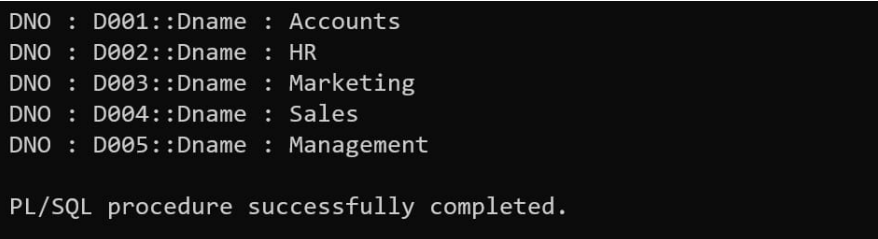
\includegraphics[scale=1]{CURSOR3.png}
%%%%%%%%%%%%%%%%%%%%%%%%%%%%%%%%%%%%%%%%%%%%%
\newpage
\begin{center}
%%Title of the Program
\large\textbf{TRIGGER}
\end{center}

\begin{flushleft}
\textbf{AIM }
\end{flushleft}
%%Insert AIM of your program here
Develop PL/SQL program to implement Trigger

\begin{flushleft}
    \textbf{Question : 1}
\end{flushleft}
Write PL/SQL trigger program to display the salary differences between the old values and new values in the table employee as per the schema

\begin{flushleft}
\textbf{QUERY }
\end{flushleft}
 \begin{verbatim}

CREATE OR REPLACE TRIGGER display_salary_changes
BEFORE DELETE OR INSERT OR UPDATE ON employeetable
FOR EACH ROW
WHEN (NEW.ID > 0)
DECLARE
sal_diff number;
BEGIN
sal_diff := :NEW.Salary - :OLD.Salary;
dbms_output.put_line(’Old salary: ’ || :OLD.salary);
dbms_output.put_line(’New salary: ’ || :NEW.salary);
dbms_output.put_line(’Salary difference: ’ || sal_diff);
END;
/
Trigger created.
DECLARE
BEGIN
UPDATE employeetable
SET Salary = Salary + 4000;
END;
/
\end{verbatim}
\begin{flushleft}
\textbf{DATABASE TABLES}
\end{flushleft}
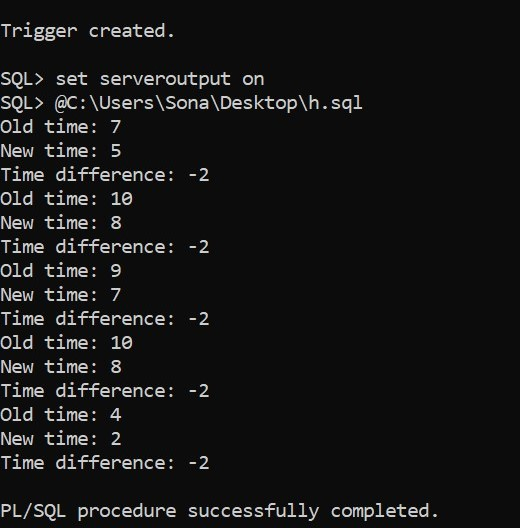
\includegraphics[scale=1]{trigger1.jpg}

\begin{flushleft}
    \textbf{Question : 2}
\end{flushleft}
Write PL/SQL trigger program to display the hour differences between the old values and new values in the table Works\_on as per the schema

\begin{flushleft}
\textbf{QUERY }
\end{flushleft}
 \begin{verbatim}
CREATE OR REPLACE TRIGGER display_hour_changes
BEFORE DELETE OR INSERT OR update on Work_on
for each row
when (NEW.HOURS > 0)
DECLARE
hour_diff number;
BEGIN
hour_diff := :NEW.HOURS - :OLD.HOURS;
dbms_output.put_line(’Old time: ’ || :OLD.HOURS);
dbms_output.put_line(’New time: ’ || :NEW.HOURS);
dbms_output.put_line(’Salary difference: ’ || hour_diff);
END;
/
Trigger created.
DECLARE
BEGIN
UPDATE Works_on
SET HOURS = HOURS - 4;
END;
/
\end{verbatim}
\begin{flushleft}
\textbf{DATABASE TABLES}
\end{flushleft}
\includegraphics[scale=1]{trigger2.jpg}

%%%%%%%%%%%%%%%%%%%%%%%%%%%%%%%%%%%%%%
\newpage
\begin{center}
%%Title of the Program
\large\textbf{TCL}
\end{center}

\begin{flushleft}
\textbf{AIM }
\end{flushleft}
%%Insert AIM of your program here
Develop SQL Queries to understand the concept of Transaction Control Language

\begin{flushleft}
    \textbf{Question : 1}
\end{flushleft}
Creating Check points in the program

\begin{flushleft}
\textbf{QUERY }
\end{flushleft}
 \begin{verbatim}
mysql> start transaction;
Query OK, 0 rows affected (0.01 sec)

mysql> savepoint save1;
Query OK, 0 rows affected (0.00 sec)

mysql> insert into Employee values("e1006","Anju","Rajesh",
"Sobha Marina,Kochi","Female",
80000,"SP1004","D005",29);
Query OK, 1 row affected (0.01 sec)

mysql> savepoint save2;
Query OK, 0 rows affected (0.00 sec)
\end{verbatim}
\begin{flushleft}
\textbf{DATABASE TABLES}
\end{flushleft}
\includegraphics[scale=0.3]{tcl1.png}
\includegraphics[scale=0.3]{tcl2.png}

\begin{flushleft}
    \textbf{Question : 2}
\end{flushleft}
Rollback to a previously created Checkpoint in the program

\begin{flushleft}
\textbf{QUERY }
\end{flushleft}
 \begin{verbatim}
mysql> rollback to save1;
Query OK, 0 rows affected (0.01 sec)

\end{verbatim}
\begin{flushleft}
\textbf{DATABASE TABLES}
\end{flushleft}
\includegraphics[scale=0.3]{tcl3.png}
\begin{flushleft}
    \textbf{Question : 3}
\end{flushleft}
Commit the program

\begin{flushleft}
\textbf{QUERY }
\end{flushleft}
 \begin{verbatim}
mysql> commit;
Query OK, 0 rows affected (0.00 sec)


\end{verbatim}
\begin{flushleft}
\textbf{DATABASE TABLES}
\end{flushleft}

\includegraphics[scale=0.4]{tcl4.png}

\newpage
\begin{center}
%%Title of the Program
\large\textbf{MongoDB}
\end{center}

\begin{flushleft}
\textbf{AIM }
\end{flushleft}
%%Insert AIM of your program here
Develop program to perform operations in MongoDB

\begin{flushleft}
    \textbf{Question : 1}
\end{flushleft}
Create a database emp

\begin{flushleft}
\textbf{QUERY }
\end{flushleft}
 \begin{verbatim}
test> use emp
\end{verbatim}
\begin{flushleft}
\textbf{DATABASE TABLES}
\end{flushleft}
\includegraphics[scale=0.464]{M1c.png}

\begin{flushleft}
    \textbf{Question : 2}
\end{flushleft}
Create new Collection
\begin{flushleft}
\textbf{QUERY }
\end{flushleft}
 \begin{verbatim}
emp> db.createCollection("Department")
{ ok: 1 }
\end{verbatim}
\begin{flushleft}
\textbf{DATABASE TABLES}
\end{flushleft}
\includegraphics[scale=0.5]{create&getM.png}
\begin{flushleft}
    \textbf{Question : 3}
\end{flushleft}
Check the collection list created and drop collection
\begin{flushleft}
\textbf{QUERY }
\end{flushleft}
 \begin{verbatim}
emp> db.getCollectionNames()
emp> db.Department.drop()
\end{verbatim}
\newpage
\begin{flushleft}
\textbf{DATABASE TABLES}
\end{flushleft}
\includegraphics[scale=0.5]{M3.png}
\begin{flushleft}
    \textbf{Question : 4}
\end{flushleft}
Insert document in selected Collection
\begin{flushleft}
\textbf{QUERY }
\end{flushleft}
 \begin{verbatim}
emp> db.Employee.insertOne({"Empno" : "E1001" , "Empname" : "Archana" ,
"Salary" : 140000})
{
  acknowledged: true,
  insertedId: ObjectId("63c51ae5fd5856e66b201526")
}
emp> try{ db.Employee.insertMany([{"Empno" : "E1002" , "Empname" : "Rahul" ,
"Salary" : 120000},{"Empno" : "E1003" , "Empname" : "Sara" , "Salary" : 170000}]);
... }
... catch(e){
... print(e);
... }
{
  acknowledged: true,
  insertedIds: {
    '0': ObjectId("63c51bb7fd5856e66b201527"),
    '1': ObjectId("63c51bb7fd5856e66b201528")
  }
}
\end{verbatim}
\newpage
\begin{flushleft}
\textbf{DATABASE TABLES}
\end{flushleft}
\includegraphics[scale=0.5]{M4.2.png}
\begin{flushleft}
    \textbf{Question : 5}
\end{flushleft}
To get the list documents in Collection
\begin{flushleft}
\textbf{QUERY }
\end{flushleft}
 \begin{verbatim}
 emp> db.Employee.find()
\end{verbatim}
\begin{flushleft}
\textbf{DATABASE TABLES}
\end{flushleft}
\includegraphics[scale=0.5]{M4.2.png}
\begin{flushleft}
    \textbf{Question : 6}
\end{flushleft}
Update the document in Collection
\begin{flushleft}
\textbf{QUERY }
\end{flushleft}
 \begin{verbatim}
emp> db.Employee.updateOne({"Empno" : "E1001"},
... {
... $set : {"Salary" : 160000},
... $currentDate : {lastModified : true}
... }
... )
{
  acknowledged: true,
  insertedId: null,
  matchedCount: 1,
  modifiedCount: 1,
  upsertedCount: 0
}
\end{verbatim}
\begin{flushleft}
\textbf{DATABASE TABLES}
\end{flushleft}
\includegraphics[scale=0.4]{M6.png}
\begin{flushleft}
    \textbf{Question : 7}
\end{flushleft}
Delete the document in selected Collection
\begin{flushleft}
\textbf{QUERY }
\end{flushleft}
 \begin{verbatim}
emp> db.Employee.deleteOne({"Empname" : "Sara"});
{ acknowledged: true, deletedCount: 1 }
\end{verbatim}
\begin{flushleft}
\textbf{DATABASE TABLES}
\end{flushleft}
\includegraphics[scale=0.4]{M8.png}
\begin{flushleft}
    \textbf{Question : 8}
\end{flushleft}
Projection using find() method
\begin{flushleft}
\textbf{QUERY }
\end{flushleft}
 \begin{verbatim}
 emp> db.Employee.find({}, {"Empname" : 1}).pretty()
\end{verbatim}
\begin{flushleft}
\textbf{DATABASE TABLES}
\end{flushleft}
\includegraphics[scale=0.386]{M9copy.png}
\begin{flushleft}
    \textbf{Question : 9}
\end{flushleft}
Drop database emp
\begin{flushleft}
\textbf{QUERY }
\end{flushleft}
 \begin{verbatim}
emp> db.dropDatabase()
\end{verbatim}
\begin{flushleft}
\textbf{DATABASE TABLES}
\end{flushleft}

\includegraphics[scale=0.53]{M10.png}
\newpage
\begin{center}
%%Title of the Program
\large\textbf{GRAPH SQL}
\end{center}

\begin{flushleft}
\textbf{AIM }
\end{flushleft}
%%Insert AIM of your program here
Develop a GraphQL program to print "Hello world"

\begin{flushleft}
    \textbf{OUTPUT}
\end{flushleft}
\includegraphics[scale=0.4]{Screenshot 2022-12-15 161337.png}
\includegraphics[scale=0.4]{Screenshot 2022-12-15 161407.png}
\includegraphics[scale=0.4]{Screenshot 2022-12-15 161435.png}
\newpage
\begin{center}
		%%Title of the Program
		\large\textbf{JAVA DATABASE CONNECTIVITY}
	\end{center}
	
	\begin{flushleft}
		\textbf{AIM }
	\end{flushleft} 
%%Insert AIM of your program here
Develop program to implement Java 
Database Connectivity

  
\begin{flushleft}
    \textbf{Question : 2}
\end{flushleft}
Write a program which connects to an online book database and insert the details of the
books in to the database.


\begin{flushleft}
\textbf{DATABASE TABLES}
\end{flushleft}
\includegraphics[scale=1]{book.png}

\begin{flushleft}
    \textbf{Question : 2}
\end{flushleft}
Write a program which connects to 
an online Employee database and 
retrieve the details of the 
employees in the database as per 
the schema.

\begin{flushleft}
\textbf{DATABASE TABLES}
\end{flushleft}
\includegraphics[scale=0.7]{sports.png}

\begin{flushleft}
	\textbf{Question : 3}
\end{flushleft}
Write a program which connects to an online hospital database and update the details of
the patients in the database.

\begin{flushleft}
	\textbf{DATABASE TABLES}
\end{flushleft}
\includegraphics[scale=0.7]{hospital.png}

\begin{flushleft}
	\textbf{Question : 4}
\end{flushleft}

Write a program which connects to an online Hotel database and delete the details of the
orders from the database.

\begin{flushleft}
	\textbf{DATABASE TABLES}
\end{flushleft}
\includegraphics[scale=0.7]{hotel.png}

\newpage
\begin{center}
	%%Title of the Program
	\large\textbf{PROJECT}
\end{center}

\begin{flushleft}
	\textbf{AIM}
\end{flushleft}
Develop an Application software using java and mySQL for an Information Management
Purpose.
\begin{flushleft}
    \textbf{PROJECT DESCRIPTION}
\end{flushleft}
Software to allocate sports venue and sports items to costumers based on the availablity. The costumers can easily view and select the required options. The software mainly aims
for providing support to sports compplexes which need to allocate it's venues properly.
	\begin{flushleft}
		\textbf{USERS AND FUNCTIONALITIES }
	\end{flushleft}
\begin{itemize}
 \item  ADMIN LOGIN
 \begin{itemize}
 	\item  Add more Venues and items.
 	\item  Remove Venues and items.
 	\item  Add more Venues.
 	\item  Remove users.
 \end{itemize}
	\item USER LOGIN
	 \begin{itemize}
		\item  Add more Venues and items to the list.
		\item  Remove Venues and items from the list.
	\end{itemize}
\end{itemize}
\begin{flushleft}
		\textbf{REFERENCE DESIGN} 
\end{flushleft} 
\big Activity diagram
\\
\includegraphics[scale=.5]{ACTIVITY.png}
\newline

\big ER DIAGRAM
\\
\includegraphics[scale=.5]{ER.png}
\newline
\big UML DIAGRAM
\\
\includegraphics[scale=1]{UML.png}
\newline

\big UI
\\
\includegraphics[scale=0.5]{SIGNUP.png}
\includegraphics[scale=0.5]{LOGIN_PAGE.png}
\includegraphics[scale=0.5]{ADMIN_PAGE.png}
\includegraphics[scale=0.5]{ADD_VENUES.png}
\newline
\begin{flushleft}
		\textbf{SOFTWARE TOOLS} 
\end{flushleft} 
Apache Netbeans\\
MySQL\\
Java\\

\begin{flushleft}
		\textbf{IMPLEMENTATION} 
\end{flushleft} 
\text{GANTT CHART}
\includegraphics[scale=1]{GANTT.png}
\begin{flushleft}
		\textbf{RESULT AND OUTPUT}
\end{flushleft} 
\includegraphics[scale=0.5]{CURRENT.png}
\includegraphics[scale=0.5]{VENUES.png}
\includegraphics[scale=0.5]{DELETE_VENUE.png}
\includegraphics[scale=0.5]{SIGNUP_PAGE.png}

\begin{flushleft}
		\textbf{CRITICAL EVALUATION} 
\end{flushleft} 
The software has been tested for varius use cases nd works properly.
\begin{flushleft}
		\textbf{CONCLUSION} 
\end{flushleft} 
It is an effecive method for proper allocation of sports items and venues in a sports complex 
\begin{flushleft}
		\textbf{REFERENCES} 
\end{flushleft} 
MySQL\\
JAVA Database Connectivity\\
JAVA Swing\\
\end{document}